\section{\texorpdfstring{$1, \zeta(2), L(2, \chi_{-3})$}{1, \textbackslash{}zeta(2), L(2, \textbackslash{}chi\_\{-3\})} 的线性无关性证明}\label{sec:13}

在本节中, 我们利用附录 A 的结果来完成定理 A 的证明. 
该证明是通过反证法进行的, 即通过证明某个特定的 G-函数不可能存在来进行. 
假设为了导出矛盾, 在周期 \(1, \zeta(2), L(2, \chi_{-3})\) 之间存在一个 \(\mathbf{Q}\)-线性关系, 
我们可以将其写为:
\begin{equation}\label{eq:13.0.1}
a + b \cdot L(2, \chi_{-3})/2 + c \cdot \zeta(2)/4 = 0
\end{equation}
对于某些不全为零的有理整数 \(a, b, c \in \mathbf{Z}\). 
命题 11.1.8 随后构造了一个具有分母类型 \([1,\dots,n]^2\) 
且在 \(\mathbf{P}^1 \setminus \{0,1/9,1,\infty\}\) 上 holonomic 延拓的特定 G-函数 \(H(x) \in \mathbf{Q}[\![x]\!]\).

现在, 第 11.2 节将该 G-函数 \(H(x)\) 转换为了在对称坐标
\[ y := x + x/(x - 1) = x^2/(x - 1) \]
下的 G-函数 \(G(y) := \operatorname{Sym}^+ H(x) \in \mathbb{Q}[\![y]\!]\). 
引理 11.2.2 表明 \(G(y) \in \mathbf{Q}[\![y]\!]\) 的分母类型为 \([1,\dots,2n]^2\). 
在另一方面, \(G(y)\) 在 \(y \in \mathbf{P}^1 \setminus \{0,4,\infty,-1/72\}\) 上是 holonomic 的, 
在 \(y \in \mathbf{C} \setminus [4,\infty)\) 上是全纯的, 
并且绕 y = 4 具有 \(\mathbf{Z}/2\) 局部单值性.

我们应用定理 6.0.2 于具有如下形式的 \(14 \times 2\) 分母类型数组：
\begin{equation}\label{eq:13.0.2}
\mathbf{b} := \begin{pmatrix} 
0 & 2 & 2 & 2 & 2 & 2 & 2 & 2 & 2 & 2 & \dots \\ 
0 & 0 & 2 & 4 & 4 & 4 & 4 & 4 & 4 & 4 & \dots
\end{pmatrix}^{\mathrm{t}}
\end{equation}
以及增加积分向量：
\[ \mathbf{e} := (0, 0, 1; 0, 0, 0, 0, 0, 0; 1, 1, 1, 1, 1), \]
该定理是在将等式中的字母 x 替换为轴对称化字母
\[ y := x + x/(x-1) = x^2/(x-1) \]
以及取以下有序函数列表 \(\{f_i\}_{i=1}^{14}\) （参见 (10.1.2), (10.1.4) 以及 (10.2.1)）的前提下浮现的:
\[ B_1(y), B_2(y), B_3(y); B_4(y), B_5(y), G(y), G'(y), G''(y), G'''(y); \]
\[ B_6(y), B_7(y), \int G(y) dy, \int \frac{G(y) - G(0)}{y} dy, \int \frac{G(y) - G(0) - G'(0)y}{y^2} dy. \]
这 14 个函数的 \(\mathbf{Q}(y)\)-线性无关性已经在引理 12.1.1 中得到证明. 
它们的分母类型已在引理 10.2.2 中被计算出来. 
对于这些积分, 我们评述：由除以 y 的方幂而引起的索引移动意味着这些函数在字面上不具有分母类型 \(n[1, 2, \ldots, 2n]^2\), 
而实际上具有分母类型 \(n[1, 2, \ldots, 2n + 3]^2\)； 
由于注记 6.0.12, 这并不是一个问题.

我们用 \(\mathcal{H}_{Y_0(2)}\) 表示由这些函数组成的 14-维 \(\mathbf{Q}(y)\)-线性生成空间. 
对于在已发展的各种 holonomy 边界中浮现的解析映射 \(\varphi\), 
我们取引理 A.4.4 中全纯映射 \(\varphi \in \mathcal{O}(\overline{\mathbf{D}})\) 的限制 \(\varphi(rz)\). 
由 \(\Sigma^0_{Y_0(2)} := \{-1/72\}\), \(\Sigma^1_{Y_0(2)} := \emptyset\), \(\varphi_{Y_0(2)} := \varphi\) 
以及为线段 [-1/72, 0] 的一个足够小的开邻域的 \(U_{Y_0(2)}\) 下使用的推论 9.0.19, 
我们拥有解析性 \(\varphi^*\mathcal{H}_{Y_0(2)} \subset \mathcal{M}(\overline{\mathbf{D}})\).

\begin{figure}[!htbp]
  \centering
  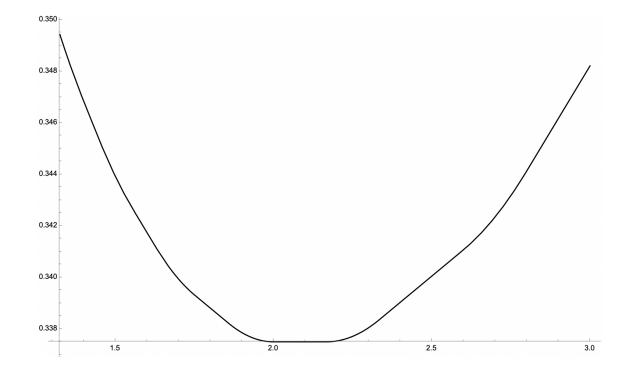
\includegraphics[width=0.45\textwidth]{assets/fig/_page_171_Figure_13.jpeg}
  \caption{\(\xi \in [1.325, 3]\) 范围内 \((6\xi + I_{\xi}^{14}(\xi))/98\) 的函数图像片段，显示区间 \(\xi \in [2, 13/6]\) 为恒定的极小值点.}\label{fig:13.0.3}
\end{figure}

对分母速率, 我们计算出:
\begin{equation}\label{eq:13.0.4}
\tau^{\flat}(\mathbf{b}) = \frac{1 \cdot 0 + (3+5) \cdot 2 + (7+9+11+13+\dots+27) \cdot 4}{14^2} = \frac{191}{49}
\end{equation}
并且, 由图~\ref{fig:13.0.3}（其揭示了 \(\xi \in [2, 13/6]\) 是一致的极大值点）:

\begin{equation}\label{eq:13.0.5}
\begin{aligned}
\tau^{\sharp}(\mathbf{e}) 
&= \frac{2}{m^{2}} \min_{\xi \in [0, m]} \left\{ \xi \sum_{i=1}^{m} e_{i} + \left( \max_{1 \le i \le m} e_{i} \right) I_{\xi}^{m}(\xi) \right\} \\
&= \min_{\xi \in [0, 14]} \left\{ \frac{6\xi + I_{\xi}^{14}(\xi)}{98} \right\} \\
&= \frac{12 + I_{2}^{14}(2)}{98} = \frac{27}{80}.
\end{aligned}
\end{equation}
我们获得:
\begin{equation}\label{eq:13.0.6}
\tau(\mathbf{b}; \mathbf{e}) = \tau^{\flat}(\mathbf{b}) + \tau^{\sharp}(\mathbf{e}) = \frac{191}{49} + \frac{27}{80} = \frac{16603}{3920} = 4.235459...
\end{equation}
这正是在公式 (A.5.1) 中浮现的数值 \(\frac{191}{49} + \frac{27}{80} = \frac{16603}{3920}\).

我们现在可以与我们的 holonomy 边界建立联系来证明定理 A. 
根据命题 11.1.8 以及引理 12.1.1, 
在假设存在 \(\mathbf{Q}\)-线性关系 \eqref{eq:13.0.1} 的前提下, 
我们拥有一组具有分母类型 \eqref{eq:13.0.2} 且在 \(\mathbf{Q}[y]\) 中在 \(\mathbf{Q}(y)\) 上线性无关的 m = 14 个（holonomic）函数. 
因此, 只要证明我们的任何一个 holonomy 边界均给出 m < 14, 就足以反驳 \eqref{eq:13.0.1}.

例如：

\begin{proof}[基于定理 7.0.1 的证明]
应用定理 7.0.1, 我们获得了上界 \(m \le 13.9938...\), 这正是公式 (A.5.1) 中计算出的.
\end{proof}

\begin{proof}[基于定理 6.0.2 的证明]
应用具有 \(l=1, r_0=e^{-1/2}, \gamma_1=14\) 的定理 6.0.2. 
由在引理 7.6.8 中类似的数值理由, 我们选取这一特定的参数. 
在此情况下, 我们有:
\[ \int_0^1 2t \cdot g_{\varphi, \gamma}^*(t) \, dt = 11.316 \dots \]
并且因此, holonomy 边界读作:
\[ m \le \frac{11.316... + \frac{1}{14} \cdot 2.926^2 \cdot \frac{1}{2}}{\log\left(256 \cdot \frac{5448339453535586608000000000}{8658833407565631122430056127}\right) - \left(\frac{27}{80} + \frac{191}{49}\right)} = 13.730... < 14. \]
\end{proof}

\begin{proof}[基于定理 7.1.6 的证明]
伴随如示例 7.4.6 中取 \(r_0 = e^{-1/2}\) 以及 \(r_1 = 1\) 的参数选择, 我们获得了边界（参见等式 (7.4.7)）.
\end{proof}

当然, 我们也可以应用第 7 节中的其他 holonomicity 边界. 
参见具有四个半径 \(r_i\) 而非两个的示例 7.4.6, 以及示例 7.5.9 以及 7.6.8.

\begin{remark}\label{rem:13.0.7}
如果我们一直坚持处于没有增加积分的、定理 2.5.1 的更粗糙框架 \(\mathbf{e} = \mathbf{0}\) 下, 
我们将不得不把 \(\mathbf{b}\) 扩充为数组:
\begin{equation}\label{eq:13.0.8}
\mathbf{b}' := \begin{pmatrix} 
0 & 2 & 2 & 2 & 2 & 2 & 2 & 2 & 2 & 2 & \dots \\ 
0 & 0 & 2 & 4 & 4 & 4 & 4 & 4 & 4 & 4 & \dots \\
0 & 0 & 0 & 0 & 0 & 0 & 0 & 0 & 2 & 2 & \dots
\end{pmatrix}^{\mathrm{t}}
\end{equation}
注意，尽管该 \(\mathbf{b}'\) 在字面上不具有定理 6.0.2 中的特定形式, 
但我们可以应用定理 8.0.1 中更一般的分母公式 \eqref{eq:8.0.2}. 
然而, 为了简单起见, 我们给出了关于 \(\tau^{\flat}(\mathbf{b}')\) 的一个足够优秀的估计, 
这足以说明引入非零 \(\mathbf{e}\) 的必要性. 
在一方面, 注记 8.0.6 中的上界论证适用于其中每一列都具有两个值（包括其中一个是 0）的那些 \(\mathbf{b}'\). 
因此我们有 \(\tau^{\flat}(\mathbf{b}') \leq (2+2+1) - \frac{1}{14^2}(1^2 \cdot 2 + 3^2 \cdot 2 + 8^2 \cdot 1) = \frac{32}{7} = 4.571...\)

在另一方面, 根据 \eqref{eq:8.0.2} 的定义, 
通过仅考虑满足 \(n_{j_1} > n_{j_2} \implies i_{j_1} \ge i_{j_2}\) 的 \(\mathbf{n}\), 我们有一个容易的下界, 
并且有 \(\tau^{\flat\flat}(\mathbf{b}')\) 至少为:
\[
\begin{aligned}
&\frac{1}{14^2} \Big( 1 \cdot 0 + 3 \cdot 2 + 5 \cdot (2 + 1) + (7 + 9 + \dots + 17) \cdot (2 + 2) \\
&\quad + (19 + 21 + 23 + 25 + 27) \cdot (2 + 2 + 1) \Big)
\end{aligned}
\]
\[ = \frac{884}{196} = 4.510\dots, \]
这是一个相比于 \eqref{eq:13.0.6} 明显更差的数值. \end{remark}